\documentclass[english,10pt]{beamer}

\mode<presentation>{
  \useinnertheme{rectangles}
  \usecolortheme[rgb={0.0,0.5,1.0}]{structure}
  \usecolortheme{orchid}
  \usecolortheme{whale}
  \useoutertheme{infolines}
  \setbeamercovered{transparent}
}

% packages
\usepackage{babel}
\usepackage[utf8]{inputenc}
\usepackage[T1]{fontenc}
\usepackage{lmodern}
\usepackage{graphicx}
\usepackage{wasysym}
\usepackage{relsize}
\usepackage{color}
\usepackage{verbatim}
\usepackage{listings}
\usepackage{algpseudocode}
\usepackage{tikz}
\usepackage{xspace}

\definecolor{version}{rgb}{1,0.5,0}

% Solarized colors
\definecolor{sbase03}{HTML}{002B36}
\definecolor{sbase02}{HTML}{073642}
\definecolor{sbase01}{HTML}{586E75}
\definecolor{sbase00}{HTML}{657B83}
\definecolor{sbase0}{HTML}{839496}
\definecolor{sbase1}{HTML}{93A1A1}
\definecolor{sbase2}{HTML}{EEE8D5}
\definecolor{sbase3}{HTML}{FDF6E3}
\definecolor{syellow}{HTML}{B58900}
\definecolor{sorange}{HTML}{CB4B16}
\definecolor{sred}{HTML}{DC322F}
\definecolor{smagenta}{HTML}{D33682}
\definecolor{sviolet}{HTML}{6C71C4}
\definecolor{sblue}{HTML}{268BD2}
\definecolor{scyan}{HTML}{2AA198}
\definecolor{sgreen}{HTML}{859900}

\lstloadlanguages{[11]C++}

\lstset{
  language=[11]C++,
  frame=lines,
  showstringspaces=false,
  xleftmargin=1ex,
  xrightmargin=1ex,
  % Light Solarized
  backgroundcolor=\color{sbase3},
  basicstyle=\ttfamily\color{sbase00},
  keywordstyle=\bfseries\color{scyan},
  commentstyle=\color{sbase1},
  stringstyle=\color{sblue},
  numberstyle=\color{sviolet},
  identifierstyle=\color{sbase00},
}

\title{Multi-Paradigm Programming}
\subtitle{Modern C++ programming}
\author{Julien BERNARD}
\institute[Univ. Franche-Comté]{Université de Franche-Comté, France}
\date{version 2025.1}

\AtBeginPart
{
  \frame{\partpage}
  \begin{frame}<beamer>
    \frametitle{Outline}
    \tableofcontents[subsubsectionstyle=hide]
  \end{frame}
}

\AtBeginSubsection[]
{
  \begin{frame}<beamer>
    \frametitle{Outline}
    \tableofcontents[currentsection,currentsubsection,subsubsectionstyle=show/show/hide/hide]
  \end{frame}
}

\AtBeginSubsubsection[]
{
  \begin{frame}<beamer>
    \frametitle{Outline}
    \tableofcontents[currentsection,currentsubsection,subsubsectionstyle=show/shaded/hide/hide]
  \end{frame}
}

\newcommand{\strong}[1]{\textbf{#1}}
\newcommand{\manualfootnote}{$^\dagger$}
\newcommand{\sourceinput}[1]{\vspace{-1ex}\smaller\lstinputlisting{#1}\larger\vspace{-1.2ex}}

\newcommand{\CCLang}{C\texttt{++}\xspace}
\newcommand{\CC}[1]{C\texttt{++}#1\xspace}
\newcommand{\Since}[1]{$^{\text{\bfseries\textcolor{version}{[C\texttt{++}#1]}}}$}

\begin{document}

\begin{frame}
  \titlepage
\end{frame}

\part{Introduction}

\section{Introduction}

\subsection{About this course}

\begin{frame}{Objective}{}
  \begin{block}{Objective}
    Learn how to use different paradigms in a single application with modern \CCLang

    \begin{itemize}
    \item
      procedural programming
    \item
      object-oriented programming
    \item
      functional programming
    \item
      generic programming
    \end{itemize}
  \end{block}
\end{frame}

\begin{frame}{Organisation}{}
  \begin{block}{Hours}
    \begin{itemize}
    \item
      Lecture: 5 $\times$ 1h30
    \item
      Test: 1 $\times$ 1h30
    \item
      Laboratory: 6 $\times$ 3h00
    \end{itemize}
  \end{block}

  \begin{block}{Evaluation}
    \begin{itemize}
    \item
      Multiple choice test (50\%)
    \item
      Laboratory project in \CCLang (50\%)
    \end{itemize}
  \end{block}
\end{frame}

\begin{frame}{Resources}{}
  \begin{block}{Online}
    \begin{itemize}
    \item
      \CCLang Reference: \url{http://en.cppreference.com/w/cpp}
    \item
      \CCLang FAQ: \url{http://isocpp.org/faq}
    \item
      \CCLang Core Guidelines: \url{https://github.com/isocpp/CppCoreGuidelines/}
    \end{itemize}
  \end{block}

  \begin{block}{Books}
    \begin{thebibliography}{}
    \bibitem{Stroustrup}
      Bjarne Stroustrup.
      \newblock {\em The \CCLang Programming Language}.
      \newblock 4th edition, 2013, Addison--Wesley
    \end{thebibliography}
  \end{block}
\end{frame}

\section{Presentation of \CCLang}

\subsection{\CCLang Origins}

% Source: "Evolving a language in and for the real world: 1991-2006", Bjarne Stroustrup

\begin{frame}{\CCLang History (1/3)}{Early \CCLang}
  \begin{block}{Early \CCLang (1979--1998)}
    \begin{itemize}
    \item
      1979: "C with Classes", Bjarne Stroustrup, AT\&T Bell Labs
    \item
      1983: "C with Classes" $\leadsto$ \CCLang; CFront 1.0
    \item
      1985: \emph{The \CCLang Programming Language}, 1st edition, Bjarne Stroustrup
    \item
      1989: \emph{The Annotated \CCLang Reference Manual}, Bjarne Stroustrup; CFront 2.0
    \item
      1991: First ISO/IEC JTC1/SC22/WG21 meeting; CFront 3.0
    \item
      1992: \emph{Effective \CCLang}, 1st edition, Scott Meyers
    \item
      1993: Standard Template Library, Alexander Stepanov, HP Labs
    \item
      1994: \emph{The Design and Evolution of \CCLang}, Bjarne Stroustrup
    \item
      1998: \emph{Effective \CCLang}, 2nd edition, Scott Meyers
    \end{itemize}
  \end{block}
\end{frame}

\begin{frame}{\CCLang History (2/3)}{Standard \CCLang}
  \begin{block}{Standard \CCLang (1998--2011)}
    \begin{itemize}
    \item
      1998: ISO standardization, \CC{98}
    \item
      2001: \emph{Modern \CCLang Design}, Andrei Alexandrescu
    \item
      2003: \CC{03}, minor revision
    \item
      2005: \emph{Effective \CCLang}, 3rd edition, Scott Meyers
    \item
      2006: Performance Technical Report
    \item
      2007: Library Technical Report 1 (TR1)
    \end{itemize}
  \end{block}
\end{frame}

\begin{frame}{\CCLang History (3/3)}{Modern \CCLang}
  \begin{block}{Modern \CCLang (2011--)}
    \begin{itemize}
    \item
      2011: \CC{11}, major revision
      \begin{itemize}
      \item[$\to$]
        "Surprisingly, \CC{11} feels like a new language"
      \end{itemize}
    \item
      2012: Standard \CCLang Foundation
    \item
      2014: \CC{14}, minor revision; \emph{Effective Modern \CCLang}, Scott Meyers
    \item
      2015: \CCLang Core Guidelines, Guidelines Support Library
    \item
      2017: \CC{17}, major revision
    \item
      2020: \CC{20}, next major revision of the standard
    \end{itemize}
  \end{block}
\end{frame}

\begin{frame}{Design Rules (1/4)}{General rules}
  \begin{block}{General rules}
    \begin{enumerate}
    \item
      \CCLang's evolution must be driven by real problems.
    \item
      Don't get involved in a sterile quest for perfection.
    \item
      \CCLang must be useful \emph{now}.
    \item
      Every feature must have a reasonably obvious implementation.
    \item
      Always provide a transition path.
    \item
      \CCLang is a language, not a complete system.
    \item
      Provide comprehensive support for each supported style.
    \item
      Don't try to force people to use a specific programming style.
    \end{enumerate}
  \end{block}
\end{frame}

\begin{frame}{Design Rules (2/4)}{Design support rules}
  \begin{block}{Design support rules}
    \begin{enumerate}
    \item
      Support sound design notions.
    \item
      Provide facilities for program organization.
    \item
      Say what you mean.
    \item
      All features must be affordable.
    \item
      It is more important to allow a useful feature than to prevent every misuse.
    \item
      Support composition of software from separately developed parts.
    \end{enumerate}
  \end{block}
\end{frame}

\begin{frame}{Design Rules (3/4)}{Language-technical rules}
  \begin{block}{Language-technical rules}
    \begin{enumerate}
    \item
      No implicit violations of the static type system.
    \item
      Provide as good support for user-defined types as for built-in types.
    \item
      Locality is good.
    \item
      Avoid order dependencies.
    \item
      If in doubt, pick the variant of a feature that is easiest to teach.
    \item
      Syntax matters (often in perverse ways).
    \item
      Preprocessor usage should be eliminated.
    \end{enumerate}
  \end{block}
\end{frame}

\begin{frame}{Design Rules (4/4)}{Low-level programming support rules}
  \begin{block}{Low-level programming support rules}
    \begin{enumerate}
    \item
      Use traditional (dumb) linkers.
    \item
      No gratuitous incompatibilities with C.
    \item
      Leave no room for a lower-level language below C++ (except assembler).
    \item
      What you don’t use, you don’t pay for (zero-overhead rule).
    \item
      If in doubt, provide means for manual control.
    \end{enumerate}
  \end{block}
\end{frame}

\subsection{\CCLang Paradigms}

\begin{frame}{Programming paradigm}{}
  \begin{definition}[Programming paradigm]
    A \strong{programming paradigm} is a way to think about the execution and/or the organization of a program. A programming paradigm enables some constructs in a language and forbids other constructs.
  \end{definition}

  \begin{block}{Remarks}
    \begin{itemize}
    \item
      There are dozens of programming paradigms.
    \item
      Most languages can be classified into multiple paradigms (like \CCLang).
    \end{itemize}
  \end{block}

  \begin{example}[Imperative programming]
    \strong{Imperative programming} is a paradigm that uses a sequence of statements to change the program's state.
  \end{example}
\end{frame}

\begin{frame}{Procedural programming}{}
  \begin{definition}[Procedural programming]
    \strong{Procedural programming} is an imperative programming paradigm based on the concept of \emph{procedure call}.
  \end{definition}
  \begin{block}{Procedural programming in \CCLang}
    \CCLang is a procedural programming language.
    \begin{itemize}
    \item
      Modularity through function parameters and return values
    \item
      Function call from any other function
    \item[$\to$]
      C style
    \end{itemize}
  \end{block}
\end{frame}

\begin{frame}{Object-oriented programming}{}
  \begin{definition}[Object-oriented programming]
    \strong{Object-oriented programming} is an imperative programming paradigm based based on the concepts of \emph{objects} (data) and \emph{methods} (code).
  \end{definition}
  \begin{block}{Object-oriented programming in \CCLang}
    \CCLang is an object-oriented programming language.
    \begin{itemize}
    \item
      Classes (\lstinline!class!)
      \begin{itemize}
      \item[$\to$]
        Class-based object-oriented programming ($\neq$ Prototype-based)
      \end{itemize}
    \item
      Composition and (multiple) inheritance
    \item
      Polymorphism (\lstinline!virtual! methods, \lstinline!dynamic_cast!)
    \end{itemize}
  \end{block}
\end{frame}

\begin{frame}{Functional programming}{}
  \begin{definition}[Functional programming]
    \strong{Functional programming} is a programming paradigm based on the concept of \emph{mathematical functions} and forbids side effects (no assignment).
  \end{definition}
  \begin{block}{Functional programming in \CCLang}
    \CCLang is \strong{not} a functional programming language\ldots
    \begin{itemize}
    \item
      No currying
    \end{itemize}
    \ldots but has elements of a functional programming language.
    \begin{itemize}
    \item
      Recursion
    \item
      Functors and lambda functions\Since{11} (closures)
    \item
      \lstinline!std::function!\Since{11}
    \end{itemize}
  \end{block}
\end{frame}

\begin{frame}{Generic programming}{}
  \begin{definition}[Generic programming]
    \strong{Generic programming} is a programming paradigm where types and algorithms are defined with abstract type parameters.
  \end{definition}
  \begin{block}{Generic programming in \CCLang}
    \CCLang is a generic programming language.
    \begin{itemize}
    \item
      Templates
    \item
      Standard Template Library (STL): containers, iterators, algorithms
    \item
      Concepts\Since{20}
    \end{itemize}
  \end{block}
\end{frame}

\begin{frame}{Using multiple paradigms}{}
  \begin{example}
    \sourceinput{snippets/multi_paradigm.cc}

    \begin{itemize}
    \item
      Procedural: \lstinline!drawAll()!
    \item
      Object-oriented: \lstinline!shape->draw()!
    \item
      Functional: \lstinline![](const Shape *shape) \{ \}!
    \item
      Generic: \lstinline!std::vector<Shape*>! and \lstinline!std::for_each!
    \end{itemize}
  \end{example}
\end{frame}


\section{Basics of \CCLang}

\subsection{Language}

\subsubsection{Value category}

%   - lvalue, rvalue, ... http://en.cppreference.com/w/cpp/language/value_category

\subsubsection{References}


\subsubsection{Exceptions}

% exception
%   http://www.drdobbs.com/when-and-how-to-use-exceptions/184401836
%   exception safety


%   - namespace
% auto, decltype
% east const, const west
% volatile
% ODR


\subsection{Standard Library}

%  new/delete -> make_unique, make_shared, vector, etc.

\part{Procedural programming}
\label{part:proc}

\section{Procedural programming}

% definition and declaration

\subsection{Arguments}

\subsubsection{Default arguments}

\begin{frame}{Default arguments}{}
  \begin{definition}[Default arguments]
    \strong{Default arguments} are used in calls where \emph{trailing} arguments are missing.
  \end{definition}

  \begin{example}[Default arguments]
    \sourceinput{snippets/default_arguments.cc}
  \end{example}
\end{frame}

\subsubsection{Variadic arguments}

\begin{frame}{Variadic arguments}{}
  \begin{definition}[Variadic arguments]
    \strong{Variadic arguments} are used when a function accepts any number of arguments. They are indicated by a parameter of the form \lstinline!...! (ellipsis) that must appear last in the parameter list of the function declaration.
  \end{definition}

  \begin{block}{Remarks}
    \begin{itemize}
    \item
      The ellipsis can be noted \lstinline!...! (\CCLang style) or \lstinline!, ...! (C style)
      \smallskip
      \sourceinput{snippets/ellipsis.cc}
    \item
      To be able to access the arguments, the function must have at least one named paramter before the ellipsis
    \end{itemize}
  \end{block}
\end{frame}

\begin{frame}{Accessing variadic arguments}{}
  \begin{block}{Accessing variadic arguments}
    The \lstinline!<cstdarg>! header provides facilities for accessing the variadic arguments:
    \begin{itemize}
    \item
      The \lstinline!va_list! type holds the information for accessing the variadic arguments
    \item
      The \lstinline!va_start! macro enables access to the variable arguments
    \item
      The \lstinline!va_arg! macro accesses the next variadic function argument
    \item
      The \lstinline!va_end! macro ends traversal of the variadic function arguments
    \end{itemize}
  \end{block}

  \begin{block}{Default argument promotions}
    \begin{itemize}
    \item
      \lstinline!nullptr_t! is converted to \lstinline!void*!
    \item
      \lstinline!float! is converted to \lstinline!double!
    \item
      \lstinline!bool!, \lstinline!char!, \lstinline!short! are converted to \lstinline!int!
    \end{itemize}
  \end{block}
\end{frame}


\begin{frame}{Example of variadic arguments}{}
  \begin{example}
    \sourceinput{snippets/variadic_arguments.cc}
  \end{example}
\end{frame}

\subsection{Overloading}

\subsubsection{Function overloading}

\begin{frame}{Function overloading}{}
  \begin{definition}[Function overloading]
    \strong{Function overloading} is the ability to create multiple functions with the same name with different implementations. Two overloaded function must differ by the type of their parameters.
  \end{definition}

  \begin{block}{Overload resolution}
    When a function is overloaded, overload resolution is the process to select the function that will be called.
    \begin{itemize}
    \item
      Determination of the set of candidate functions after name lookup and template argument deduction
    \item
      Determination of the set of viable functions after examining arguments and parameters
    \item
      Choice of the best viable function
    \end{itemize}
    Overload resolution may fail and result in a compilation error.
  \end{block}
\end{frame}

\begin{frame}{Function overloading}{}
  \begin{example}[Function overloading]
    \sourceinput{snippets/overload.cc}
  \end{example}
\end{frame}

\subsubsection{Operator overloading}

\begin{frame}{Operator overloading}{}
  \begin{block}{Operator overloading}
    Operator overloading is a special case of function overloading. Operators that can be overloaded are:
    \begin{itemize}
    \item
      Arithmetic operators: \lstinline!+!, \lstinline!-!, \lstinline!*!, \lstinline!/!, \lstinline!\%!, \lstinline!\^!, \lstinline!\&!, \lstinline!|!, \lstinline!\~!, \lstinline!<<!, \lstinline!>>!
    \item
      Increment and decrement operators: \lstinline!++!, \lstinline!--!
    \item
      Logical operators: \lstinline+!+, \lstinline!&&!, \lstinline!||!
    \item
      Assignment operators: \lstinline!=!, \lstinline!+=!, \lstinline!-=!, \lstinline!*=!, \lstinline!/=!, \lstinline!\%=!, \lstinline!\^=!, \lstinline!\&=!, \lstinline!|=!, \lstinline!<<=!, \lstinline!>>=!
    \item
      Comparisons operators: \lstinline!==!, \lstinline+!=+, \lstinline!<!, \lstinline!>!, \lstinline!<=!, \lstinline!>=!, \lstinline!<=>!\Since{20}
    \item
      Access operators: \lstinline!->!, \lstinline!->*!, \lstinline![]!
    \item
      Special operators: \lstinline!,! (comma), \lstinline!()! (call)
    \end{itemize}
  \end{block}
\end{frame}

\begin{frame}{Overloaded operators}{}
  \begin{block}{Overloaded operators}
    \begin{center}
      \scriptsize
      \begin{tabular}{|c|c|c|l|}
        \hline
        Expression & Member function & Free function & Example \\
        \hline
        \lstinline!@a! & \lstinline!(a).operator@()! & \lstinline!operator@(a)! & \lstinline+!std::cin+ \\
                      &                             &                          & $\to$ \lstinline+std::cin.operator!()+ \\
        \hline
        \lstinline!a @ b! & \lstinline!(a).operator@(b)! & \lstinline!operator@(a,b)! & \lstinline!std::cout << 42! \\
                          &                              &                            & $\to$ \lstinline!std::cout.operator<<(42)! \\
        \hline
        \lstinline!a = b! & \lstinline!(a).operator=(b)! &                            & \lstinline!std::string s; s = "abc";! \\
                          &                              &                            & $\to$ \lstinline!std::string.operator=("abc")! \\
        \hline
        \lstinline!a(b)! & \lstinline!(a).operator()(b)! &                            & \lstinline!std::random_device r; auto n = r();! \\
                        &                               &                            & $\to$ \lstinline!r.operator()()! \\
        \hline
        \lstinline!a[b]! & \lstinline!(a).operator[](b)! &                            & \lstinline!std::map<int, int> m; m[1] = 2;! \\
                        &                               &                            & $\to$ \lstinline!m.operator[](1)! \\
        \hline
        \lstinline!a->!  & \lstinline!(a).operator->()!  &                            & \lstinline!auto p = std::make_unique<S>(); p->bar()! \\
                        &                               &                            & $\to$ \lstinline!p.operator->()! \\
        \hline
        \lstinline!a@!   & \lstinline!(a).operator@(0)!  & \lstinline!operator@(a,0)! & \lstinline!auto i = v.begin(); i++! \\
                        &                               &                            & $\to$ \lstinline!i.operator++(0)! \\
        \hline
      \end{tabular}
    \end{center}
  \end{block}
\end{frame}

\begin{frame}{Restrictions on overloaded operators}{}
  \begin{block}{Restrictions on overloaded operators}
    \begin{itemize}
    \item
      The following operators can \strong{not} be overloaded:
      \begin{itemize}
      \item
        \lstinline!::! (scope resolution)
      \item
        \lstinline!.! (member access)
      \item
        \lstinline!.*! (member access through pointer to member)
      \item
        \lstinline!?:! (ternary conditional)
      \end{itemize}
    \item
      New operators such as \lstinline!**!, \lstinline!<>!, or \lstinline!&|! can \strong{not} be created
    \item
      The overloads of operators \lstinline!&&! and \lstinline!||! lose short-circuit evaluation
    \item
      The overload of operator \lstinline!->! must either return a raw pointer, or return an object (by reference or by value) for which operator \lstinline!->! is in turn overloaded
    \item
      It is \strong{not} possible to change:
      \begin{itemize}
      \item
        the precedence of operators
      \item
        the grouping of operators
      \item
        the number of operands of operators
      \end{itemize}
    \end{itemize}
  \end{block}
\end{frame}

\begin{frame}{Operator overloading}{}
  \begin{example}[Operator overloading]
    \sourceinput{snippets/overload_operator.cc}
  \end{example}
\end{frame}

\subsection{Parameter passing}

% https://isocpp.github.io/CppCoreGuidelines/CppCoreGuidelines#Rf-conventional

\begin{frame}{Properties of types}{}
  \begin{block}{Properties of types}
    Types may be of three kinds regarding their ease of use in functions:
    \begin{enumerate}
    \item
      Easy types:
      \begin{itemize}
      \item
        Cheap to copy: \lstinline!int! and all fundamental types, \lstinline!std::tuple<bool, int*>!, \ldots
      \item
        Impossible to copy: \lstinline!std::unique_ptr<T>!, \ldots
      \end{itemize}
    \item
      Medium types:
      \begin{itemize}
      \item
        Cheap to move: \lstinline!std::string!, \lstinline!std::vector<T>!, \ldots
      \item
        Quite cheap to move: \lstinline!BigData!, \lstinline!std::array<std::vector<T>,N>!, \ldots
      \item
        Unknown cost: \lstinline!unknown::Type!, \ldots
      \end{itemize}
    \item
      Hard types:
      \begin{itemize}
      \item
        Expensive to move: \lstinline!std::array<BigData,N>!, \ldots
      \end{itemize}
    \end{enumerate}
  \end{block}
\end{frame}

\begin{frame}{Output only values}{}
  \begin{block}{Output only values}
    For output only values, prefer:
    \begin{itemize}
    \item
      Return values for easy and medium types \\
      \lstinline!X f();!
%       \begin{itemize}
%       \item
%         In case of multiple return values, use a \lstinline!struct! or \lstinline!std::tuple! \\
%         \lstinline!std::tuple<X,Y> f();!
%       \end{itemize}
    \item
      Output parameter (reference to non-const) for hard types \\
      \lstinline!void f(X& out);!
    \end{itemize}
  \end{block}

  \begin{example}[Output only values]
    \sourceinput{snippets/parameter_passing_out.cc}
  \end{example}
\end{frame}

\begin{frame}{Input only values}{}
  \begin{block}{Input only values}
    For input only values, prefer:
    \begin{itemize}
    \item
      Passing by value for easy types \\
      \lstinline!void f(T in);!
    \item
      Passing by const reference for medium and hard types
      \lstinline!void f(const T& in);!
    \end{itemize}
  \end{block}

  \begin{example}[Input only values]
    \sourceinput{snippets/parameter_passing_in.cc}
  \end{example}
\end{frame}

\begin{frame}{Input/Output values}{}
  \begin{block}{Input/Output values}
    For input/output values, prefer:
    \begin{itemize}
    \item
      Passing by reference to non-const for any type \\
      \lstinline!void f(T& inout);!
    \end{itemize}
  \end{block}

  \begin{example}[Input/Output values]
    \sourceinput{snippets/parameter_passing_inout.cc}
  \end{example}
\end{frame}

% parameter passing and reference


\subsection{Argument-dependent lookup}

% http://en.cppreference.com/w/cpp/language/adl

\subsection{Constant expression functions}

% constexpr

% UDL
% string ids

% mangling

% copy elision


% \begin{frame}{}{}
%   \begin{block}{}
%     \begin{itemize}
%     \item
%     \item
%     \end{itemize}
%   \end{block}
% \end{frame}

\part{Object-Oriented Programming (1/2)}
\label{part:oop1}

\section{Object-Oriented Programming -- Class, Constructor, Destructor}

\subsection{Class}

% Source: https://en.cppreference.com/w/cpp/language/classes
\begin{frame}{Class}{}
  \begin{definition}[Class]
    A \strong{class} is a user-defined type whose declaration begins with \lstinline!class! or \lstinline!struct!.
  \end{definition}

  \begin{block}{Remark}
    \lstinline!struct! and \lstinline!class! are indistinguishable in C++, except that the default access mode and default inheritance mode are \lstinline!public! if class declaration uses \lstinline!struct! and \lstinline!private! if the class declaration uses \lstinline!class!.
  \end{block}
\end{frame}


% Source: https://en.cppreference.com/w/cpp/language/classes
\begin{frame}{Class members}{}
  \begin{block}{Class members}
    A class can have the following kinds of members:
    \begin{enumerate}
    \item
      Data members
      \begin{itemize}
      \item
        Non-static data members, including bit fields
      \item
        Static data members (\lstinline!static!)
      \end{itemize}
    \item
      Member functions
      \begin{itemize}
      \item
        Non-static member functions
      \item
        Static member functions (\lstinline!static!)
      \end{itemize}
    \item
      Nested types
      \begin{itemize}
      \item
        Nested classes and enumerations defined within the class definition
      \item
        Aliases of existing types, defined with \lstinline!typedef! or type alias declarations
      \end{itemize}
    \item
      Enumerators from all unscoped enumerations defined within the class
    \item
      Member templates (variable\Since{14}, class or function templates)
    \end{enumerate}
  \end{block}
\end{frame}

\begin{frame}{Class members}{}
  \begin{example}[Class members]
    \sourceinput{snippets/class_members.cc}
  \end{example}
\end{frame}


\subsection{Constructors}

\subsubsection{Constructor and member initializer list}

% Source: https://en.cppreference.com/w/cpp/language/initializer_list
\begin{frame}{Constructor}{}
  \begin{definition}[Constructor]
    A \strong{constructor} is a special non-static member function of a class that is used to initialize objects of its class type.
  \end{definition}

  \begin{block}{Remarks}
    \begin{itemize}
    \item
      Constructors have no names and cannot be called directly
    \item
      They are invoked when initialization takes place
    \end{itemize}
  \end{block}

  \begin{block}{Special kinds of constructors}
    \begin{itemize}
    \item
      Converting constructors (without \lstinline!explicit! specifier)
    \item
      Default constructor (without arguments)
    \item
      Copy constructor and move constructor (with another object of the same type as the argument)
    \end{itemize}
  \end{block}
\end{frame}

% Source: https://en.cppreference.com/w/cpp/language/initializer_list
\begin{frame}{Initialization order}{}
  \begin{block}{Initialization order}
    \begin{enumerate}
    \item
      Initialization of virtual bases
      \begin{itemize}
      \item
        Only in the most derived class of the object that's being constructed
      \item
        In depth-first left-to-right traversal of the base class declarations
      \end{itemize}
    \item
%       \label{lst:initbase}
      Initialization of direct bases
      \begin{itemize}
      \item
        In left-to-right order
      \end{itemize}
    \item
%       \label{lst:initdatamembers}
      Initialization of non-static data members
      \begin{itemize}
      \item
        In order of declaration in the class definition
      \end{itemize}
    \item
      Execution of the body of the constructor
    \end{enumerate}
%     Step~\ref{lst:initbase} to \ref{lst:initdatamembers} can be done in the \emph{member initializer list}.
  \end{block}

  % TODO: default member initializer
\end{frame}


% Source: https://en.cppreference.com/w/cpp/language/initializer_list
\begin{frame}{Member initializer list}{}
  \begin{definition}[Member initializer list]
    In the definition of a constructor of a class, a \strong{member initializer list} specifies the \emph{non-default} initializers for direct and virtual base subobjects and non-static data members.
  \end{definition}

  \begin{block}{Remark}
    The list may not be in the same order as the members but compilers issue a warning in that case.
  \end{block}
\end{frame}

\begin{frame}{Member initializer list}{}
  \begin{example}[Member initializer list]
    \sourceinput{snippets/member_initializer_list.cc}
  \end{example}
\end{frame}

\subsubsection{Converting constructor}

% Source: https://en.cppreference.com/w/cpp/language/converting_constructor
\begin{frame}{Converting constructor and explicit constructors}{}
  \begin{definition}[Converting constructor]
    A \strong{converting constructor} is not declared with the specifier \lstinline!explicit!
  \end{definition}

  \begin{block}{Converting constructors and explicit constructors}
    \begin{itemize}
    \item
      Both kind of constructors are considered in direct initialization
    \item
      Converting constructors are also considered in copy initialization (conversion)
    \end{itemize}
  \end{block}
\end{frame}

\begin{frame}{Converting constructor}{}
  \begin{example}[Converting constructor]
    \sourceinput{snippets/converting_constructor.cc}
  \end{example}
\end{frame}

\begin{frame}{Explicit constructor}{}
  \begin{example}[Explicit constructor]
    \sourceinput{snippets/explicit_constructor.cc}
  \end{example}
\end{frame}

\subsubsection{Default constructor}

% Source: https://en.cppreference.com/w/cpp/language/default_constructor
\begin{frame}{Default constructor}{}
  \begin{definition}[Default constructor]
    A \strong{default constructor} is a constructor that can be called with no arguments (either defined with an empty parameter list, or with default arguments provided for every parameter).
  \end{definition}

  \begin{block}{Default constructor}
    \begin{itemize}
    \item
      If no user-declared constructors of any kind are provided for a class, the compiler will always declare a default constructor
    \item
      A default constructor can be:
      \begin{itemize}
      \item
        Explicitely declared with \lstinline! = default! after its declaration
      \item
        Explicitely deleted with \lstinline! = delete! after its declaration
      \end{itemize}
    \end{itemize}
  \end{block}
\end{frame}

\begin{frame}{Default constructor}{}
  \begin{example}[Default constructor]
    \sourceinput{snippets/default_constructor.cc}
  \end{example}
\end{frame}


\subsubsection{Copy/move constructor/assignment}

% Source: https://en.cppreference.com/w/cpp/language/copy_constructor
\begin{frame}{Copy constructor}{}
  \begin{definition}[Copy constructor]
    A \strong{copy constructor} of class \lstinline!T! is a non-template constructor whose parameter is (generally) \lstinline!const T&!
  \end{definition}

  \begin{block}{Copy constructor}
    \begin{itemize}
    \item
      If a copy constructor is not declared, it is implicitly declared, if possible or it is implicitly deleted otherwise
    \item
      A copy constructor can be:
      \begin{itemize}
      \item
        Explicitely declared and defaulted with \lstinline! = default! after its declaration
      \item
        Explicitely deleted with \lstinline! = delete! after its declaration
      \end{itemize}
    \item
      A copy constructor is used in the following cases (\lstinline!a! and \lstinline!b! are of type \lstinline!T!):
      \begin{itemize}
      \item
        Initialization: \lstinline!T a = b;! or \lstinline!T a(b);!
      \item
        Function argument passing: \lstinline!f(a);!, where \lstinline!f! is \lstinline!void f(T t)!
      \item
        Function return: \lstinline!return a;! inside a function such as \lstinline!T f()!, where type \lstinline!T! has no move constructor
      \end{itemize}
    \end{itemize}
  \end{block}
\end{frame}

% Source: https://en.cppreference.com/w/cpp/language/move_constructor
\begin{frame}{Move constructor}{}
  \begin{definition}[Move constructor]
    A \strong{move constructor} of class \lstinline!T! is a non-template constructor whose parameter is (generally) \lstinline!T&&!
  \end{definition}

  \begin{block}{Move constructor}
    \begin{itemize}
    \item
      If a move constructor is not declared, it is implicitly declared, if possible or it is implicitly deleted otherwise
    \item
      A move constructor can be:
      \begin{itemize}
      \item
        Explicitely declared and defaulted with \lstinline! = default! after its declaration
      \item
        Explicitely deleted with \lstinline! = delete! after its declaration
      \end{itemize}
    \item
      A move constructor is used in the following cases (\lstinline!a! and \lstinline!b! are of type \lstinline!T!):
      \begin{itemize}
      \item
        Initialization: \lstinline!T a = std::move(b);! or \lstinline!T a(std::move(b));!
      \item
        Function argument passing: \lstinline!f(std::move(a));!, where \lstinline!f! is \lstinline!void f(T t)!
      \item
        Function return: \lstinline!return a;! inside a function such as \lstinline!T f()!, where type \lstinline!T! has a move constructor
      \end{itemize}
    \end{itemize}
  \end{block}
\end{frame}

\begin{frame}{Copy and move constructors}{}
  \begin{example}[Copy and move constructors]
    \sourceinput{snippets/copy_move_constructors.cc}
  \end{example}
\end{frame}

% Source: https://en.cppreference.com/w/cpp/language/copy_assignment
\begin{frame}{Copy assignment}{}
  \begin{definition}[Copy assignment]
    A \strong{copy assignment operator} of class \lstinline!T! is a non-template non-static member function with the name \lstinline!operator=! and whose parameter is (generally) \lstinline!const T&! and whose return type is \lstinline!T&!
  \end{definition}

  \begin{block}{Copy assignment}
    \begin{itemize}
    \item
      If a copy assignment is not declared, it is implicitly declared, if possible or it is implicitly deleted otherwise
    \item
      A copy assignment can be:
      \begin{itemize}
      \item
        Explicitely declared and defaulted with \lstinline! = default! after its declaration
      \item
        Explicitely deleted with \lstinline! = delete! after its declaration
      \end{itemize}
    \end{itemize}
  \end{block}
\end{frame}

% Source: https://en.cppreference.com/w/cpp/language/move_assignment
\begin{frame}{Move assignment}{}
  \begin{definition}[Move assignment]
    A \strong{move assignment operator} of class \lstinline!T! is a non-template non-static member function with the name \lstinline!operator=! and whose parameter is (generally) \lstinline!T&&! and whose return type is \lstinline!T&!
  \end{definition}

  \begin{block}{Move assignment}
    \begin{itemize}
    \item
      If a move assignment is not declared, it is implicitly declared, if possible or it is implicitly deleted otherwise
    \item
      A move assignment can be:
      \begin{itemize}
      \item
        Explicitely declared and defaulted with \lstinline! = default! after its declaration
      \item
        Explicitely deleted with \lstinline! = delete! after its declaration
      \end{itemize}
    \end{itemize}
  \end{block}
\end{frame}

\begin{frame}{Copy and move assignment}{}
  \begin{block}{Copy and move assignment}
    If both copy and move assignment operators are provided, overload resolution selects:
    \begin{itemize}
    \item
      the move assignment if the argument is an \emph{rvalue} (either a \emph{prvalue} such as a nameless temporary or an \emph{xvalue} such as the result of \lstinline!std::move!),
    \item
      the copy assignment if the argument is an \emph{lvalue} (named object or a function/operator returning lvalue reference)
    \end{itemize}
    If only the copy assignment is provided, all argument categories select it (as long as it takes its argument by value or as reference to const, since rvalues can bind to const references), which makes copy assignment the fallback for move assignment, when move is unavailable.
  \end{block}
\end{frame}

\begin{frame}{Copy and move assignments}{}
  \begin{example}[Copy and move assignments]
    \sourceinput{snippets/copy_move_assignments.cc}
  \end{example}
\end{frame}


\subsection{Destructors}

\subsubsection{Destructor}

% Source: https://en.cppreference.com/w/cpp/language/destructor
\begin{frame}{Destructor}{}
  \begin{definition}[Destructor]
    A \strong{destructor} is a special member function that is called when the lifetime of an object ends. The purpose of the destructor is to free the resources that the object may have acquired during its lifetime.

    {
      \hfill\lstinline[mathescape]!\~ $ClassName$ ()!\hfill
    }
  \end{definition}

  \begin{block}{Destruction sequence}
    \begin{enumerate}
    \item
      Execution of the body of the destructor
    \item
      Destruction of non-static data members
      \begin{itemize}
      \item
        In reverse order of declaration in the class definition
      \end{itemize}
    \item
      Destruction of direct bases
      \begin{itemize}
      \item
        In reverse order of construction, i.e. right-to-left
      \end{itemize}
    \item
      Destruction of virtual bases
      \begin{itemize}
      \item
        Only in the most derived class of the object that's being destroyed
      \end{itemize}
    \end{enumerate}
  \end{block}
\end{frame}

% Source: https://en.cppreference.com/w/cpp/language/destructor
\begin{frame}{Destructor call}{}
  \begin{block}{Destructor call}
    The destructor is called whenever an object's lifetime ends, which includes:
    \begin{itemize}
    \item
      program termination, for objects with static storage duration
    \item
      thread exit, for objects with thread-local storage duration
    \item
      end of scope, for objects with automatic storage duration and for temporaries whose life was extended by binding to a reference
    \item
      delete expression, for objects with dynamic storage duration
    \item
      end of the full expression, for nameless temporaries
    \item
      stack unwinding, for objects with automatic storage duration when an exception escapes their block, uncaught
    \item[$\to$]
      Most of the time, the destructor is called automatically!
    \end{itemize}
  \end{block}
\end{frame}

\begin{frame}{Destructor}{}
  \begin{example}[Destructor]
    \sourceinput{snippets/destructor.cc}
  \end{example}
\end{frame}


\subsubsection{Rule of Three, Rule of Five, Rule of Zero}

% Source: https://en.cppreference.com/w/cpp/language/rule_of_three
\begin{frame}{Rule of Three}{}
  \begin{definition}[Rule of Three]
    If a class requires
    \begin{itemize}
    \item
      a user-defined destructor,
    \item
      a user-defined copy constructor,
    \item
      or a user-defined copy assignment operator,
    \end{itemize}
    it almost certainly requires all three.
  \end{definition}

  \begin{block}{Reason}
    The implicitly-defined special member functions are typically incorrect if the class is managing a resource whose handle is an object of non-class type (raw pointer, POSIX file descriptor, etc), whose destructor does nothing and copy constructor/assignment operator performs a "shallow copy" (copy the value of the handle, without duplicating the underlying resource).
  \end{block}
\end{frame}

\begin{frame}{Rule of Three}{}
  \begin{example}[Rule of Three]
    \sourceinput{snippets/rule_of_three.cc}
  \end{example}
\end{frame}

% Source: https://en.cppreference.com/w/cpp/language/rule_of_three
\begin{frame}{Rule of Five}{}
  \begin{definition}[Rule of Five]
    Because the presence of a user-defined destructor, copy-constructor, or copy-assignment operator prevents implicit definition of the move constructor and the move assignment operator, any class for which move semantics are desirable, has to declare all five special member functions
  \end{definition}

  \begin{block}{Remark}
    Unlike Rule of Three, failing to provide move constructor and move assignment is usually not an error, but a missed optimization opportunity.
  \end{block}
\end{frame}

\begin{frame}{Rule of Five}{}
  \begin{example}[Rule of Five]
    \sourceinput{snippets/rule_of_five.cc}
  \end{example}
\end{frame}

% Source: https://en.cppreference.com/w/cpp/language/rule_of_three
\begin{frame}{Rule of Zero}{}
  \begin{definition}[Rule of Zero]
    Classes that have custom destructors, copy/move constructors or copy/move assignment operators should deal exclusively with ownership (which follows from the Single Responsibility Principle). Other classes should not have custom destructors, copy/move constructors or copy/move assignment operators.
  \end{definition}
\end{frame}

\begin{frame}{Rule of Zero}{}
  \begin{example}[Rule of Zero]
    \sourceinput{snippets/rule_of_zero.cc}
  \end{example}
\end{frame}

\subsubsection{Resource Acquisition Is Initialization (RAII)}

% Source: https://en.cppreference.com/w/cpp/language/raii
\begin{frame}{Resource Acquisition Is Initialization (RAII)}{}
  \begin{definition}[Resource Acquisition Is Initialization (RAII)]
    \strong{Resource Acquisition Is Initialization} (RAII), is a C++ programming technique which binds the life cycle of a resource that must be acquired before use to the lifetime of an object.
  \end{definition}

  \begin{examples}[Resources where RAII could be used]
    \begin{itemize}
    \item
       Allocated heap memory
    \item
       Thread of execution
    \item
       Open socket
    \item
       Open file
    \item
       Locked mutex
    \item
       Disk space
    \item
       Database connection
    \end{itemize}
  \end{examples}
\end{frame}

% Source: https://en.cppreference.com/w/cpp/language/raii
\begin{frame}{RAII in Practice}{}
  \begin{block}{RAII in Practice}
    \begin{itemize}
    \item
      Encapsulate each resource into a class, where
      \begin{itemize}
      \item
        the constructor acquires the resource and establishes all class invariants or throws an exception if that cannot be done
      \item
        the destructor releases the resource and never throws exceptions
      \end{itemize}
    \item
      Always use the resource via an instance of a RAII-class that either
      \begin{itemize}
      \item
        has automatic storage duration or temporary lifetime itself, or
      \item
        has lifetime bounded by the lifetime of an automatic or temporary object
      \end{itemize}
    \end{itemize}
  \end{block}

  \begin{block}{Remark}
    Classes with \lstinline!open()!/\lstinline!close()!, \lstinline!lock()!/\lstinline!unlock()!, or \lstinline!init()!/\lstinline!destroy()! member functions are typical examples of non-RAII classes
  \end{block}
\end{frame}

\begin{frame}{Resource Acquisition Is Initialization}{}
  \begin{example}[Resource Acquisition Is Initialization]
    \sourceinput{snippets/raii.cc}
  \end{example}
\end{frame}

% - Others might be more helpful in grokking what it really is, such as "Constructor Acquires, Destructor Releases" (CADRe) or "Scope-based Resource Management" (SBRM).

\part{Object-Oriented Programming (2/2)}
\label{part:oop2}

\section{Object-Oriented Programming -- Inheritance, Polymorphism, Idioms}

\subsection{Inheritance}

\subsubsection{Derived classes}

% Source: https://en.cppreference.com/w/cpp/language/derived_class
\begin{frame}{Derived Classes}{}
  \begin{block}{Derived Classes}
    Any class may be declared as \emph{derived} from one or more \emph{base classes} which, in turn, may be derived from their own base classes, forming an inheritance hierarchy. Each base class:
    \begin{itemize}
    \item
      may have an access specifer: \lstinline!public!, \lstinline!protected!, \lstinline!private!
    \item
      may be declared \lstinline!virtual!
    \end{itemize}
  \end{block}

  \begin{block}{Remark}
    If the access specifier is omitted, it defaults to:
    \begin{itemize}
    \item
      \lstinline!public! for \lstinline!struct!
    \item
      \lstinline!private! for \lstinline!class!
    \end{itemize}
  \end{block}
\end{frame}

\begin{frame}{Derived Classes}{}
  \begin{example}[Derived Classes]
    \sourceinput{snippets/derived_class.cc}
  \end{example}
\end{frame}


\begin{frame}{Inheritance and member access}{}
  \begin{block}{Inheritance and member access}
    \begin{center}
      \lstinline[mathescape]!struct B \{ \}; struct D : $\;specifier\;$ B \{ \};!

      \bigskip

      \begin{tabular}{|c|c|c|c|}
      \hline
      Inheritance           & \multicolumn{3}{|c|}{Member in \lstinline!B!} \\
      \lstinline[mathescape]!$specifier$! & \lstinline!public!    & \lstinline!protected! & \lstinline!private! \\
      \hline
      \lstinline!public!    & \lstinline!public!    & \lstinline!protected! & - \\
      \lstinline!protected! & \lstinline!protected! & \lstinline!protected! & - \\
      \lstinline!private!   & \lstinline!private!   & \lstinline!private!   & - \\
      \hline
      \end{tabular}

      Member access in \lstinline!D!
    \end{center}
  \end{block}
\end{frame}

\subsubsection{Virtual base classes}

% Source: https://en.cppreference.com/w/cpp/language/derived_class
\begin{frame}{Virtual base class}{}
  \begin{block}{Virtual base class}
    For each distinct base class that is specified \lstinline!virtual!, the most derived object contains only one base class subobject of that type, even if the class appears many times in the inheritance hierarchy (as long as it is inherited \lstinline!virtual! every time).
  \end{block}

  \begin{example}[Famous example of virtual base class]
    \begin{center}
    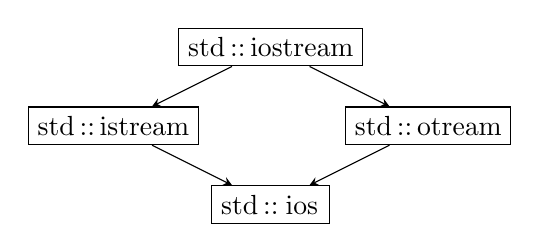
\begin{tikzpicture}
      \node[draw] (IO) at ( 0, 0) { \lstinline!std::iostream! } ;
      \node[draw] (I) at (-2,-1) { \lstinline!std::istream! } ;
      \node[draw] (O) at ( 2,-1) { \lstinline!std::otream! } ;
      \node[draw] (B) at ( 0,-2) { \lstinline!std::ios! } ;

      \draw[->,>=stealth] (IO) -- (I) ;
      \draw[->,>=stealth] (IO) -- (O) ;
      \draw[->,>=stealth] (I) -- (B) ;
      \draw[->,>=stealth] (O) -- (B) ;
    \end{tikzpicture}
    \end{center}
  \end{example}
\end{frame}

\begin{frame}{Virtual base class}{}
  \begin{example}[Virtual base class]
    \sourceinput{snippets/virtual_base_class.cc}
  \end{example}
\end{frame}

% TODO: initialization of virtual base class?


\subsubsection{Empty Base Optimization (EBO)}

% Source: https://en.cppreference.com/w/cpp/language/ebo
\begin{frame}{Empty Base Optimization (EBO)}{}
  \begin{block}{Empty Base Optimization (EBO)}
    \strong{Empty Base Optimization} (EBO) allows the size of an empty base subobject to be zero
  \end{block}

  \begin{block}{Explanation}
    \begin{itemize}
    \item
      The size of any object or member subobject is required to be at least 1 even if the type is an empty class, in order to be able to guarantee that the addresses of distinct objects of the same type are always distinct.
    \item
      However, base class subobjects are not so constrained, and can be completely optimized out from the object layout
    \end{itemize}
  \end{block}
\end{frame}

\begin{frame}{Empty Base Optimization}{}
  \begin{example}[Empty Base Optimization]
    \sourceinput{snippets/ebo.cc}
  \end{example}
\end{frame}


\subsection{Polymorphism}

\subsubsection{Virtual functions}

% Source: https://en.cppreference.com/w/cpp/language/virtual
\begin{frame}{Virtual functions}{}
  \begin{definition}[Virtual function]
    A \strong{virtual function} is a non-static member function with the \lstinline!virtual! specifier. A virtual function supports dynamic dispatch, i.e. its behavior can be overridden in derived classes.
  \end{definition}

  \begin{block}{Virtual functions override}
    A function that overrides a virtual function in a derived class must have the same:
    \begin{itemize}
    \item
      name
    \item
      parameter type list (but not the return type)
    \item
      cv-qualifiers and ref qualifiers
    \end{itemize}
  \end{block}

  \begin{block}{Remark}
    A virtual function does not need to be visible (\lstinline!public! or \lstinline!protected!) to be overridden.
  \end{block}
\end{frame}

\begin{frame}{Virtual functions}{}
  \begin{example}[Virtual functions]
    \sourceinput{snippets/virtual_functions.cc}
  \end{example}
\end{frame}

% Source: https://en.cppreference.com/w/cpp/language/virtual
\begin{frame}{\texttt{override} and \texttt{final}}{}
  \begin{block}{\texttt{override} and \texttt{final}}
    \begin{itemize}
    \item
      If a function is declared with the specifier \lstinline!override!, but does not override a virtual function, the program is ill-formed
    \item
      If a function is declared with the specifier \lstinline!final!, and another function attempts to override it, the program is ill-formed
    \end{itemize}
  \end{block}
\end{frame}

\begin{frame}{\texttt{override} and \texttt{final}}{}
  \begin{example}[\texttt{override} and \texttt{final}]
    \sourceinput{snippets/override_and_final.cc}
  \end{example}
\end{frame}

\subsubsection{Virtual destructors}

% Source: https://en.cppreference.com/w/cpp/language/virtual
\begin{frame}{Virtual destructor}{}
  \begin{block}{Virtual destructor}
    Even though destructors are not inherited, if a base class declares its destructor virtual, the derived destructor always overrides it. This makes it possible to delete dynamically allocated objects of polymorphic type through pointers to base.
  \end{block}
  \begin{block}{Important remark}
    If a class is polymorphic (declares or inherits at least one virtual function), it must declare its destructor private.
  \end{block}
\end{frame}

\begin{frame}{Virtual destructor}{}
  \begin{example}[Virtual destructor]
    \sourceinput{snippets/virtual_destructor.cc}
  \end{example}
\end{frame}

\subsubsection{Pure virtual functions}

% Source: https://en.cppreference.com/w/cpp/language/abstract_class
\begin{frame}{Pure virtual functions and abstract classes}{}
  \begin{definition}[Pure virtual function]
    A \strong{pure virtual function} is a virtual function with the \emph{pure specifier} noted \lstinline!= 0!.
  \end{definition}

  \begin{definition}[Abstract class]
    An \strong{abstract class} is a class that either defines or inherits at least one pure virtual function.
  \end{definition}

  \begin{block}{Remarks}
    \begin{itemize}
    \item
      No objects of an abstract class can be created
    \item
      Abstract classes are used as base classes for concrete classes
    \end{itemize}
  \end{block}
\end{frame}

\begin{frame}{Pure virtual functions and abstract classes}{}
  \begin{example}[Abstract class]
    \sourceinput{snippets/abstract_class.cc}
  \end{example}
\end{frame}

\subsubsection{Virtual table}

% Source: https://en.wikipedia.org/wiki/Virtual_method_table
\begin{frame}{Virtual table and virtual table pointer}{}
  \begin{definition}[Virtual table]
    A \strong{virtual table} (or vtable) is a per-class table containing function pointers to virtual functions. It is generated by the compiler.
  \end{definition}

  \begin{definition}[Virtual table pointer]
    A \strong{virtual table pointer} (or vptr) is a per-object pointer to a virtual table added by the constructor. The vptr is part of the object.
  \end{definition}

  \begin{block}{Call to a virtual function}
    \begin{enumerate}
    \item
      Fetch the virtual table pointer of the object
    \item
      Call the function declared in the table pointed by the virtual table pointer
    \end{enumerate}
    Consequence: calling a virtual function requires an indirection!
  \end{block}
\end{frame}

\begin{frame}{Virtual table and virtual table pointer}{}
  \begin{example}[Virtual table and virtual table pointer]
    \sourceinput{snippets/vtable_vptr.cc}
  \end{example}
\end{frame}

\subsubsection{Run-time type information (RTTI)}

% Source: https://en.cppreference.com/w/cpp/language/dynamic_cast
\begin{frame}{\texttt{dynamic\_cast}}{}
  \begin{block}{\texttt{dynamic\_cast}}
    A \strong{\lstinline!dynamic_cast!} safely converts pointers and references to classes up, down, and sideways along the inheritance hierarchy.

    {
      \hfill\lstinline[mathescape]!dynamic_cast<$type$>($expr$)!\hfill
    }

    \lstinline[mathescape]!$expr$! is:
    \begin{itemize}
    \item
      A glvalue of a complete class type if \lstinline[mathescape]!$type$! is a reference
    \item
      A prvalue of a pointer to a complete class type if \lstinline[mathescape]!$type$! is a pointer
    \end{itemize}
  \end{block}

  \begin{block}{Result of a \texttt{dynamic\_cast}}
    \begin{itemize}
    \item
      If the cast is successful, \lstinline!dynamic_cast! returns a value of type \lstinline[mathescape]!$type$!.
    \item
      If the cast fails and \lstinline[mathescape]!$type$! is a pointer type, it returns a null pointer.
    \item
      If the cast fails and \lstinline[mathescape]!$type$! is a reference type, it throws an exception that matches a handler of type \lstinline!std::bad_cast!.
    \end{itemize}
  \end{block}
\end{frame}

\begin{frame}{\texttt{dynamic\_cast}}{}
  \begin{example}[\texttt{dynamic\_cast}]
    \sourceinput{snippets/dynamic_cast.cc}
  \end{example}
\end{frame}

% Source: https://en.cppreference.com/w/cpp/language/typeid
\begin{frame}{\texttt{typeid}}{}
  \begin{block}{\texttt{typeid}}
    The \lstinline!typeid! operator queries information of a type and returns an object of type \lstinline!const std::type_info&!. It can be used:
    \begin{itemize}
    \item
      with a type
    \item
      with an expression
    \end{itemize}
  \end{block}

  \begin{block}{\texttt{typeid} with an expression}
    \begin{itemize}
    \item
      If the expression is a glvalue expression that identifies an object of a polymorphic type, the \lstinline!typeid! expression evaluates the expression and then refers to the \lstinline!std::type_info! object that represents the dynamic type of the expression
    \item
      If expression is not a glvalue expression of polymorphic type, \lstinline!typeid! does not evaluate the expression, and the \lstinline!std::type_info! object it identifies represents the static type of the expression
    \end{itemize}
  \end{block}
\end{frame}

\begin{frame}{\texttt{typeid}}{}
  \begin{example}[\texttt{typeid}]
    \sourceinput{snippets/typeid.cc}
  \end{example}
\end{frame}

\subsection{Idioms}

\subsubsection{PImpl My Ride}

% Source: https://en.cppreference.com/w/cpp/language/pimpl
% Source: https://cpppatterns.com/patterns/pimpl.html
% Source: https://wiki.qt.io/D-Pointer
\begin{frame}{PImpl: Pointer to Implementation}{}
  \begin{block}{PImpl: Pointer to Implementation}
    \strong{PImpl} (Pointer to Implementation) (a.k.a. d-pointer or opaque pointer) is a technique to hide implemntation details of a class in order to achieve ABI stability.
  \end{block}

  \begin{block}{PImpl in practice}
    \sourceinput{snippets/pimpl.cc}
  \end{block}
\end{frame}

\begin{frame}{PImpl or not PImpl}{}
  \begin{block}{Advantages of PImpl}
    \begin{itemize}
    \item
      Compilation firewall: a modification in \lstinline!Impl! does not require a recompilation of all classes that use \lstinline!Foo!
    \item
      Move-friendly: a \lstinline!std::unique_ptr! is easy to move, especially in containers
    \end{itemize}
  \end{block}
  \begin{block}{Drawbacks of PImpl}
    \begin{itemize}
    \item
      Access overhead: an access to a member requires an indirection through a pointer
    \item
      Space overhead: the object requires an additional pointer
    \item
      Lifetime management: the implementation object is allocated on the heap
    \item
      Maintenance overhead: all the implementation has to be in a dedicated file
    \end{itemize}
  \end{block}
\end{frame}


\subsubsection{\texttt{const} correctness}

% Source: https://isocpp.org/wiki/faq/const-correctness
\begin{frame}{\texttt{const} correctness}{}
  \begin{block}{\texttt{const} correctness}
    \lstinline!const! correctness is a set of rules to offer a guarantee about the (non-)mutability of object:
    \begin{itemize}
    \item
      Choose reference to \lstinline!const! or pointer to \lstinline!const! for parameters if you do not intend to modify the parameters
    \item
      Make a member function \lstinline!const! if the function does not modify the object
    \item
      If a member function is \lstinline!const! and returns a reference to a member, the reference should be \lstinline!const! or the function should return by value
    \end{itemize}
  \end{block}

  \begin{block}{Benefits of \texttt{const} correctness}
    \begin{itemize}
    \item
      The caller has the guarantee that a variable or an object will not be modified
    \item
      The compiler ensures that the callee respects the contract by emitting an error in case of modification of a \lstinline!const! object
    \item
      The \lstinline!const! property is spread through member function calls
    \end{itemize}
  \end{block}
\end{frame}

% overload const/non-const
\begin{frame}{\texttt{const} correctness}{}
  \begin{example}[\texttt{const} correctness]
    \sourceinput{snippets/const_correctness.cc}
  \end{example}
\end{frame}



% (N)RVO

\part{Functional programming}

\section{Functional programming}

\subsection{Functional programming}

% Source: https://en.wikipedia.org/wiki/Functional_programming
\begin{frame}{Functional programming}{}
  \begin{block}{Functional programming concepts}
    \begin{itemize}
    \item
      First-class and high order functions $\to$ \lstinline!std::function!
    \item
      Pure functions $\to$ \lstinline!constexpr!
    \item
      Recursion $\to$ OK
    \item
      Strict or lazy evaluation $\to$ strict!
    \item
      Type system $\to$ KO!
    \item
      Referential transparency $\to$ KO! (\lstinline!operator=!)
    \item[$\to$]
      \CCLang is not really a functional programming language
    \end{itemize}
  \end{block}
\end{frame}


\subsection{Function objects}

% Source: https://en.cppreference.com/w/cpp/named_req/FunctionObject
\begin{frame}{Function object}{}
  \begin{definition}[Function object]
    A \strong{function object} is an object that can be used on the left of the function call operator
  \end{definition}

  \begin{block}{Function objects}
    \begin{itemize}
    \item
      Function pointer
    \item
      Object of a class with an overloaded \lstinline!operator()!
    \end{itemize}
  \end{block}
\end{frame}


\begin{frame}{Call operator}{}
  \begin{block}{Call operator}
    The call operator \lstinline!operator()! can be overloaded in any class
    \begin{itemize}
    \item
      it can take any number of arguments
    \item
      it can return anything
    \end{itemize}
  \end{block}

  \begin{block}{Remark}
    A function object can have a state
  \end{block}
\end{frame}

\begin{frame}{Function object}{}
  \begin{example}[Function object]
    \sourceinput{snippets/function_object.cc}
  \end{example}
\end{frame}

\subsection{Lambda expressions}

% Source: https://en.cppreference.com/w/cpp/language/lambda
\begin{frame}{Lambda expressions}{}
  \begin{definition}[Lambda expressions]
    A \strong{lambda expression} is a prvalue of unique class type (closure type) that provides an unamed function object capable of capturing variables in scope (closure).
  \end{definition}

  \begin{block}{Lambda expressions}
    {
      \hfill\lstinline[mathescape]![$\;captures\;$]($\;params\;$) \{ $\;body\;$ \}! or \lstinline[mathescape]![$\;captures\;$]($\;params\;$) -> $\;ret\;$ \{ $\;body\;$ \}!\hfill
    }
    \begin{itemize}
    \item
      \lstinline[mathescape]!$captures$! is a comma-separated list of captures
    \item
      \lstinline[mathescape]!$params$! is the list of parameters, as any function
      \begin{itemize}
      \item
        The type of a parameter can be \lstinline!auto!\Since{14} $\to$ generic lambda
      \end{itemize}
    \item
      \lstinline[mathescape]!$ret$! is the return type, if not present it is implied by the function return statements (or \lstinline!void! if it does not return any value)
    \end{itemize}
  \end{block}
\end{frame}

% Source: https://en.cppreference.com/w/cpp/language/lambda
\begin{frame}{Captures}{}
  \begin{block}{Captures}
    The \lstinline[mathescape]!$captures$! is a comma-separated list of zero or more captures, optionally beginning with the capture default. The only capture defaults are:

    \begin{itemize}
    \item
      \lstinline!&! (implicitly capture the used automatic variables by reference)
    \item
      \lstinline!=! (implicitly capture the used automatic variables by copy).
    \end{itemize}

    An individual capture can be:

    \begin{itemize}
    \item
      \lstinline[mathescape]!$identifier$! (simple by-copy capture)
    \item
      \lstinline[mathescape]!$identifier\;$ = $\;initializer$! (by-copy capture with initializer\Since{14})
    \item
      \lstinline[mathescape]!&$identifier$! (simple by-reference capture)
    \item
      \lstinline[mathescape]!&$identifier\;$ = $\;initializer$! (by-reference capture with initializer\Since{14})
    \item
      \lstinline[mathescape]!this! (simple by-reference capture of the current object)
    \item
      \lstinline[mathescape]!*this! (simple by-copy capture of the current object\Since{17})
    \end{itemize}
  \end{block}
\end{frame}

\begin{frame}{Lambda expressions}{}
  \begin{example}[Lambda expressions]
    \sourceinput{snippets/lambda_expression.cc}
  \end{example}
\end{frame}

\begin{frame}{Lambda expressions with capture default}{}
  \begin{example}[Lambda expressions with capture default]
    \sourceinput{snippets/lambda_expression_with_default.cc}
  \end{example}
\end{frame}

\begin{frame}{Conversion of a lambda expression}{}
  \begin{block}{Conversion of a lambda expression}
    A capture-less lambda expression can be converted to a function pointer.
  \end{block}

  \begin{example}[Lambda expressions]
    \sourceinput{snippets/lambda_conversion.cc}
  \end{example}
\end{frame}


\subsection{Generic function}

% Source: https://en.cppreference.com/w/cpp/named_req/Callable
\begin{frame}{Callable type}{}
  \begin{definition}[Callable type]
    A \strong{callable type} is a type \lstinline!T! for which the \lstinline!INVOKE! operation is applicable
  \end{definition}

  \begin{block}{Callable types}
    Given \lstinline!f! an object of type \lstinline!T!, \lstinline[mathescape]!INVOKE(f, $t_1$, $t_2$, $\ldots$, $t_N$)! is equivalent to:
    \begin{itemize}
    \item
      If \lstinline!f! is a pointer to member function of class \lstinline!T!:
      \begin{itemize}
      \item
        If \lstinline[mathescape]!$t_1$! is of type \lstinline!T!, \lstinline[mathescape]!($t_1$.*f)($t_2$, $\ldots$, $t_N$)!
      \item
        If \lstinline[mathescape]!$t_1$! is a specialization of \lstinline!std::reference_wrapper!, \\ \hfill \lstinline[mathescape]!($t_1$.get().*f)($t_2$, $\ldots$, $t_N$)!\Since{17}
      \item
        Otherwise, \lstinline[mathescape]!((*$t_1$).*f)($t_2$, $\ldots$, $t_N$)!
      \end{itemize}
    \item
      If \lstinline!f! is a pointer to data member of class \lstinline!T! and $N = 1$:
      \begin{itemize}
      \item
        If \lstinline[mathescape]!$t_1$! is of type \lstinline!T!, \lstinline[mathescape]!$t_1$.*f!
      \item
        If \lstinline[mathescape]!$t_1$! is a specialization of \lstinline!std::reference_wrapper!, \lstinline[mathescape]!$t_1$.get().*f!\Since{17}
      \item
        Otherwise, \lstinline[mathescape]!(*$t_1$).*f!
      \end{itemize}
    \item
      If \lstinline!f! is a function object, \lstinline[mathescape]!f($t_1$, $t_2$, $\ldots$, $t_N$)!
    \end{itemize}
  \end{block}
\end{frame}

% Source: https://en.cppreference.com/w/cpp/language/operator_member_access
% Source: https://en.cppreference.com/w/cpp/language/pointer#Pointers_to_data_members
\begin{frame}{Pointer to member}{}
  \begin{block}{Pointer to member access}
    The member access operator expressions through pointers to members have one of the two forms:
    \begin{itemize}
    \item
      \lstinline[mathescape]!$lhs$.*$rhs$! if \lstinline[mathescape]!$lhs$! is of class type \lstinline!T!
    \item
      \lstinline[mathescape]!$lhs$->*$rhs$! if \lstinline[mathescape]!$lhs$! is of type pointer to class type \lstinline!T!
    \end{itemize}
    \lstinline[mathescape]!$rhs$! is an expression of type pointer to member (data or function)
  \end{block}

  \begin{block}{Pointer to member}
    A pointer to non-static member \lstinline!x! (data or function) which is a member of class \lstinline!C! can be initialized with the expression \lstinline!&C::x! exactly.
  \end{block}
\end{frame}


\begin{frame}{Pointer to member}{}
  \begin{example}[Pointer to member]
    \sourceinput{snippets/pointer_to_member.cc}
  \end{example}
\end{frame}

\begin{frame}{Callable in the standard library}{}
  \begin{block}{Callable in the standard library}
    \begin{itemize}
    \item
      Types:
      \begin{itemize}
      \item
        \lstinline!std::function! can store any callable
      \item
        \lstinline!std::reference_wrapper! can store a reference to any callable
      \item
        \lstinline!std::packaged_task! can store any callable (invoked asynchronously)
      \end{itemize}
    \item
      Functions that accepts any callable:
      \begin{itemize}
      \item
        \lstinline!std::bind!
      \item
        \lstinline!std::thread::thread!
      \item
        \lstinline!std::call_once!
      \item
        \lstinline!std::async!
      \end{itemize}
    \end{itemize}
  \end{block}
\end{frame}

% Source: https://en.cppreference.com/w/cpp/utility/functional/function
\begin{frame}{\texttt{std::function}}{}
  \begin{example}[\texttt{std::function}]
    \sourceinput{snippets/std_function.cc}
  \end{example}
\end{frame}

% Source: https://en.cppreference.com/w/cpp/utility/functional/bind
\begin{frame}{Partial application}{}
  \begin{block}{Partial application}
    \lstinline!std::bind! can be used for partial application of a function. More precisely, \lstinline[mathescape]!std::bind(f, $a_1$, $\ldots$, $a_n$)! generates a forwarding call wrapper for a callable object \lstinline!f!. Calling this wrapper is equivalent to invoking \lstinline!f! with some of its arguments bound to the arguments of \lstinline!std::bind! and unbound arguments replaced by the placeholders \lstinline!_1!, \lstinline!_2!, \lstinline!_3!, etc. of namespace \lstinline!std::placeholders!.
  \end{block}

  \begin{block}{Remark}
    The arguments to \lstinline!std::bind! are copied or moved, and are never passed by reference unless wrapped in \lstinline!std::ref! or \lstinline!std::cref!.
  \end{block}
\end{frame}

\begin{frame}{Partial application}{}
  \begin{example}[Partial application]
    \sourceinput{snippets/std_bind.cc}
  \end{example}
\end{frame}

\begin{frame}{Partial application}{}
  \begin{example}[Partial application]
    \sourceinput{snippets/std_bind_pointer_to_member.cc}
  \end{example}
\end{frame}


% \subsection{Monadic types}?
% std::optional?

\subsection{High-order functions}

\begin{frame}{High-order functions}{}
  \begin{definition}[High-order function]
    A \strong{high-order function} is a function that does at least one of the following:
    \begin{itemize}
    \item
      takes one or more functions as arguments
    \item
      return a function as its result
    \end{itemize}
  \end{definition}
  \begin{block}{High-order functions}
    The three most well-known high-order functions are:
    \begin{itemize}
    \item
      \texttt{map} $\to$ \lstinline!std::transform!
    \item
      \texttt{fold} $\to$ \lstinline!std::accumulate!
    \item
      \texttt{filter} $\to$ \lstinline!std::copy_if!
    \end{itemize}
  \end{block}
\end{frame}

% Source: https://en.cppreference.com/w/cpp/algorithm/transform
\begin{frame}{\texttt{std::transform}}{}
  \begin{example}[\texttt{std::transform}]
    \sourceinput{snippets/std_transform.cc}
  \end{example}
\end{frame}

% Source: https://en.cppreference.com/w/cpp/algorithm/accumulate
\begin{frame}{\texttt{std::accumulate}}{}
  \begin{example}[\texttt{std::accumulate}]
    \sourceinput{snippets/std_accumulate.cc}
  \end{example}
\end{frame}

% Source: https://en.cppreference.com/w/cpp/algorithm/copy
\begin{frame}{\texttt{std::copy\_if}}{}
  \begin{example}[\texttt{std::copy\_if}]
    \sourceinput{snippets/std_copy_if.cc}
  \end{example}
\end{frame}


% \begin{frame}{}{}
%   \begin{block}{}
%     \begin{itemize}
%     \item
%     \item
%     \end{itemize}
%   \end{block}
% \end{frame}

\part{Generic programming}

% type traits
%
% SFINAE
%
% https://en.wikipedia.org/wiki/Curiously_recurring_template_pattern
%
% policy based programming

% https://en.cppreference.com/w/cpp/language/dependent_name


% \part{Extras}

% Things that were in previous parts but were put here because the parts
% were already too long


\section{Introduction}

\subsection{Design Rules}

\begin{frame}{Design Rules (1/4)}{General rules}
  \begin{block}{General rules}
    \begin{enumerate}
    \item
      \CCLang's evolution must be driven by real problems.
    \item
      Don't get involved in a sterile quest for perfection.
    \item
      \CCLang must be useful \emph{now}.
    \item
      Every feature must have a reasonably obvious implementation.
    \item
      Always provide a transition path.
    \item
      \CCLang is a language, not a complete system.
    \item
      Provide comprehensive support for each supported style.
    \item
      Don't try to force people to use a specific programming style.
    \end{enumerate}
  \end{block}
\end{frame}

\begin{frame}{Design Rules (2/4)}{Design support rules}
  \begin{block}{Design support rules}
    \begin{enumerate}
    \item
      Support sound design notions.
    \item
      Provide facilities for program organization.
    \item
      Say what you mean.
    \item
      All features must be affordable.
    \item
      It is more important to allow a useful feature than to prevent every misuse.
    \item
      Support composition of software from separately developed parts.
    \end{enumerate}
  \end{block}
\end{frame}

\begin{frame}{Design Rules (3/4)}{Language-technical rules}
  \begin{block}{Language-technical rules}
    \begin{enumerate}
    \item
      No implicit violations of the static type system.
    \item
      Provide as good support for user-defined types as for built-in types.
    \item
      Locality is good.
    \item
      Avoid order dependencies.
    \item
      If in doubt, pick the variant of a feature that is easiest to teach.
    \item
      Syntax matters (often in perverse ways).
    \item
      Preprocessor usage should be eliminated.
    \end{enumerate}
  \end{block}
\end{frame}

\begin{frame}{Design Rules (4/4)}{Low-level programming support rules}
  \begin{block}{Low-level programming support rules}
    \begin{enumerate}
    \item
      Use traditional (dumb) linkers.
    \item
      No gratuitous incompatibilities with C.
    \item
      Leave no room for a lower-level language below C++ (except assembler).
    \item
      What you don’t use, you don’t pay for (zero-overhead rule).
    \item
      If in doubt, provide means for manual control.
    \end{enumerate}
  \end{block}
\end{frame}


\section*{The end}

\subsection*{That's all folks!}

\begin{frame}{That's all for now\ldots}{}
  \begin{block}{}
    \begin{center}
      Questions?
    \end{center}
  \end{block}
\end{frame}


% \begin{frame}{}{}
%   \begin{block}{}
%     \begin{itemize}
%     \item
%     \item
%     \end{itemize}
%   \end{block}
% \end{frame}

\end{document}
